%% This is file `DEMO-TUDaThesis.tex' version 2.09 (2020/03/13),
%% it is part of
%% TUDa-CI -- Corporate Design for TU Darmstadt
%% ----------------------------------------------------------------------------
%%
%%  Copyright (C) 2018--2020 by Marei Peischl <marei@peitex.de>
%%
%% ============================================================================
%% This work may be distributed and/or modified under the
%% conditions of the LaTeX Project Public License, either version 1.3c
%% of this license or (at your option) any later version.
%% The latest version of this license is in
%% http://www.latex-project.org/lppl.txt
%% and version 1.3c or later is part of all distributions of LaTeX
%% version 2008/05/04 or later.
%%
%% This work has the LPPL maintenance status `maintained'.
%%
%% The Current Maintainers of this work are
%%   Marei Peischl <tuda-ci@peitex.de>
%%   Markus Lazanowski <latex@ce.tu-darmstadt.de>
%%
%% The development respository can be found at
%% https://github.com/tudace/tuda_latex_templates
%% Please use the issue tracker for feedback!
%%
%% ============================================================================
%%
% !TeX program = lualatex
%%

\documentclass[
	ngerman,
	ruledheaders=section,%Ebene bis zu der die Überschriften mit Linien abgetrennt werden, vgl. DEMO-TUDaPub
	class=report,% Basisdokumentenklasse. Wählt die Korrespondierende KOMA-Script Klasse
	thesis={type=master},% Dokumententyp Thesis, für Dissertationen siehe die Demo-Datei DEMO-TUDaPhd
	accentcolor=1b,% Auswahl der Akzentfarbe
	custommargins=true,% Ränder werden mithilfe von typearea automatisch berechnet
	marginpar=false,% Kopfzeile und Fußzeile erstrecken sich nicht über die Randnotizspalte
	%BCOR=1mm,%Bindekorrektur, falls notwendig
	parskip=half-,%Absatzkennzeichnung durch Abstand vgl. KOMA-Sript
	fontsize=11pt,%Basisschriftgröße laut Corporate Design ist mit 9pt häufig zu klein
	DIV=14,
%	logofile=example-image, %Falls die Logo Dateien nicht vorliegen
]{tudapub}


% Der folgende Block ist nur bei pdfTeX auf Versionen vor April 2018 notwendig
%\usepackage{iftex}
%\ifPDFTeX
%	\usepackage[utf8]{inputenc}%kompatibilität mit TeX Versionen vor April 2018
%\fi

%%%%%%%%%%%%%%%%%%%
%Sprachanpassung & Verbesserte Trennregeln
%%%%%%%%%%%%%%%%%%%
\usepackage[english, main=ngerman]{babel}
\usepackage[autostyle]{csquotes}% Anführungszeichen vereinfacht
\usepackage{microtype}
\usepackage[super]{nth} % converts Dec \nth{1} to Dec 1st (with st as superscript)


%%%%%%%%%%%%%%%%%%%
%Literaturverzeichnis
%%%%%%%%%%%%%%%%%%%
\usepackage[style=authoryear-ibid,backend=biber]{biblatex}   % Literaturverzeichnis
\DeclareLanguageMapping{ngerman}{ngerman-apa}
\bibliography{references}
\AtBeginBibliography{\setcounter{maxnames}{10}} % Im Literaturverzeichnis nenne mehr als 2 Autoren
\counterwithout{footnote}{chapter} % Zähle Fußnoten über gesamtes Dokument hoch


%%%%%%%%%%%%%%%%%%%
%Paketvorschläge Tabellen
%%%%%%%%%%%%%%%%%%%
%\usepackage{array}     % Basispaket für Tabellenkonfiguration, wird von den folgenden automatisch geladen
\usepackage{tabularx}   % Tabellen, die sich automatisch der Breite anpassen
\usepackage{longtable} % Mehrseitige Tabellen
\usepackage{xtab,afterpage}
%\usepackage{xltabular} % Mehrseitige Tabellen mit anpassarer Breite
\usepackage{booktabs}   % Verbesserte Möglichkeiten für Tabellenlayout über horizontale Linien
\usepackage{tikz}       % Graphen zeichnen
\usepackage{enumitem, hyperref}   % for referencing in enumerate und description
\usepackage{amsmath}    % https://tex.stackexchange.com/questions/32140/how-to-write-a-function-piecewise-with-bracket-outside
% https://texblog.org/2012/03/21/cross-referencing-list-items/
\usepackage[acronym,shortcuts,nonumberlist,nomain]{glossaries} % for Abbreviations (Acronyms)

%%%%%%%%%%%%%%%%%%%
%Paketvorschläge Mathematik
%%%%%%%%%%%%%%%%%%%
%\usepackage{mathtools} % erweiterte Fassung von amsmath
%\usepackage{amssymb}   % erweiterter Zeichensatz
%\usepackage{siunitx}   % Einheiten

% Customs
%\usepackage[singlespacing]{setspace}
\usepackage[]{setspace}
%\usepackage[printonlyused]{acronym}

%Formatierungen für Beispiele in diesem Dokument. Im Allgemeinen nicht notwendig!
\let\file\texttt
\let\code\texttt
\let\tbs\textbackslash

\usepackage{pifont}% Zapf-Dingbats Symbole
\newcommand*{\FeatureTrue}{\ding{52}}
\newcommand*{\FeatureFalse}{\ding{56}}

\makeglossaries

\begin{document}

\Metadata{
	title=Titel des Dokuments Format je nach Länge 2 oder 3-zeilig,
	author=Max Mustermann
}

\pagenumbering{gobble}

\title{Titel des Dokuments Format je nach Länge 2 oder 3-zeilig}

\studentID{12345678}
\author[M. Musterman]{Max Musterman}%optionales Argument ist die Signatur,
\birthplace{}%Geburtsort, bei Dissertationen zwingend notwendig
\reviewer{Prof. Dr. Peter Buxmann \and Prof. Dr. X Y}%Gutachter

%Diese Felder erden untereinander auf der Titelseite platziert.
%\department ist eine notwendige Angabe, siehe auch dem Abschnitt `Abweichung von den Vorgaben für die Titelseite'
\department{wi} % Das Kürzel wird automatisch ersetzt und als Studienfach gewählt, siehe Liste der Kürzel im Dokument.
\institute{Wirtschatsinformatik}
\group{Software \& Digital Business}

\submissiondate{\today}
\examdate{\today}

%	\tuprints{urn=1234,printid=12345}
%	\dedication{Für alle, die \TeX{} nutzen.}

\maketitle

\affidavit


%---------------------------------------------------------------------%
%----------------------------- Abstract ------------------------------%
%---------------------------------------------------------------------%
\chapter*{Abstract}
Der Abstract fasst den Inhalt der Abschlussarbeit auf maximal einer halben Seite zusammen. Ziel des Abstracts ist es, dem Leser einen möglichst schnellen Überblick über den Inhalt der Arbeit zu verschaffen und die wesentlichen Ergebnisse darzustellen. Mögliche Inhalte sind die Zielsetzung oder Forschungsfrage der Arbeit, verwendete Theorien, die verwendete Methodik sowie eine kurze Darstellung der zentralen Ergebnisse und Beiträge.

\tableofcontents


\pagenumbering{Roman}

%---------------------------------------------------------------------%
%-------------------------- List of Figures --------------------------%
%---------------------------------------------------------------------%

\listoffigures
\addcontentsline{toc}{chapter}{Abbildungsverzeichnis}           %Kapitel bekommt keine Nummerierung und wird trotzdem
                                                                %ins Inhaltsverzeichnis aufgenommen
%---------------------------------------------------------------------%
%--------------------------- List of Tables --------------------------%
%---------------------------------------------------------------------%

\listoftables
\addcontentsline{toc}{chapter}{Tabellenverzeichnis}           %Kapitel bekommt keine Nummerierung und wird trotzdem
                                                                %ins Inhaltsverzeichnis aufgenommen

%---------------------------------------------------------------------%
%----------------------- List of Abbreviations -----------------------%
%---------------------------------------------------------------------%
\chapter*{Abkürzungsverzeichnis}
\addcontentsline{toc}{chapter}{Abkürzungsverzeichnis}           %Kapitel bekommt keine Nummerierung und wird trotzdem
                                                                %ins Inhaltsverzeichnis aufgenommen

\begin{xtabular}{ll}
IS					&	Information Systems\\
TUD						&	Technische Universität Darmstadt\\

\end{xtabular} 

%---------------------------------------------------------------------%
%---------------------------- Introduction ---------------------------%
%---------------------------------------------------------------------%

\onehalfspacing
\chapter{Einleitung}
% Umstellen auf arabische Seitenzahlen. Die Anzahl der bisherigen
% Seiten wird zwischengespeichert, da die römische Nummerierung am
% Ende des Dokuments fortgesetzt werden soll.
\newcounter{seitenzahlroemisch}
\setcounter{seitenzahlroemisch}{\value{page}}
\pagenumbering{arabic}


Die Datei \file{DEMO-TUDaThesis.tex} ist ein Template für Abschlussarbeiten im Stil des Corporate Designs der TU Darmstadt.
Sie ist Teil des TUDa-CI-Bundles wurde vom in Teilen tuddesign-Paket von C.~v.~Loewenich und J.~Werner inspiriert.

 \section{Abbildungen}
Abbildungen sollten generell linksbündig in das Dokument eingefügt werden. Die Abbildungs-beschriftung steht dabei unter der Abbildung und ist ebenfalls linksbündig auszurichten. Eine Beschriftung der Abbildungen mit der Abkürzung "Abb." ist ebenfalls möglich. Abbildungen (bzw. ihre Beschriftungen) werden von einer Leerzeile gefolgt, um den Abstand zum nachfolgenden Text zu wahren.

Beispiele:

 
\begin{figure}[ht]
     \centering
     
\includegraphics[]{images/Picture 1.png}
     \caption{Logo des Fachgebiets Wirtschaftsinformatik}
     \label{fig:logo}
\end{figure}

\begin{figure}[ht]
     \centering
     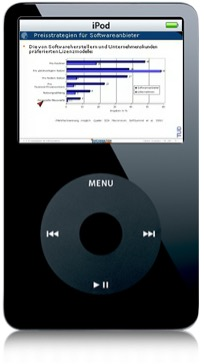
\includegraphics[]{images/Picture 1.jpg}
     \caption{Video-Podcast der Vorlesung Internet Economics auf einem iPod}
     \label{fig:logo2}
\end{figure}

\section{Zitierungen}
Wörtliche Zitate, die sich über mind. drei Textzeilen erstrecken, sind mit der "Zitat" zu formatieren. Alle anderen Zitate erhalten die gleiche Formatierung wie der restliche Fließtext \parencite{buxmann2015softwareindustrie}.

%---------------------------------------------------------------------%
%---------------------------- Conclusion -----------------------------%
%---------------------------------------------------------------------%
\chapter{Zusammenfassung und Fazit}
Lorem ipsum dolor sit amet, consetetur sadipscing elitr, sed diam nonumy eirmod tempor invidunt ut labore et dolore magna aliquyam erat, sed diam voluptua. At vero eos et accusam et justo duo dolores et ea rebum. Stet clita kasd gubergren, no sea takimata sanctus est Lorem ipsum dolor sit amet. Lorem ipsum dolor sit amet, consetetur sadipscing elitr, sed diam nonumy eirmod tempor invidunt ut labore et dolore magna aliquyam erat, sed diam voluptua. At vero eos et accusam et justo duo dolores et ea rebum. Stet clita kasd gubergren, no sea takimata sanctus est Lorem ipsum dolor sit amet. Lorem ipsum dolor sit amet, consetetur sadipscing elitr, sed diam nonumy eirmod tempor invidunt ut labore et dolore magna aliquyam erat, sed diam voluptua. At vero eos et accusam et justo duo dolores et ea rebum. Stet clita kasd gubergren, no sea takimata sanctus est Lorem ipsum dolor sit amet.
\section{Blindtext Überschrift Ebene 2 Blindheit per Definition}
Mit Blindheit per Definition geschlagen, dennoch nicht unsichtbar, präsentiere ich mich als unbeachtetes und ungeliebtes Stiefkind zeitgenössischer Literatur. Meine Bestimmung liegt - wie ich selbst - in engen Grenzen und ist rein platzhalterischer Natur. Kann ein missbrauchtes Wortgefüge eigentlich noch Schlimmeres erleiden, als als Blindtext erdacht und vor der Öffentlichkeit versteckt zu werden?
\subsection{Blindtext Überschrift Ebene 3}
Ut wisi enim ad minim veniam, quis nostrud exerci tation ullamcorper suscipit lobortis nisl ut aliquip ex ea commodo consequat. Duis autem vel eum iriure dolor in hendrerit in vulputate velit esse molestie consequat, vel illum dolore eu feugiat nulla facilisis at vero eros et accumsan et iusto odio dignissim qui blandit praesent luptatum zzril delenit augue duis dolore te feugait nulla facilisi.\\
Nam liber tempor cum soluta nobis eleifend option congue nihil imperdiet doming id quod mazim placerat facer possim assum. Lorem ipsum dolor sit amet, consectetuer adipiscing elit, sed diam nonummy nibh euismod tincidunt ut laoreet dolore magna aliquam erat volutpat. Ut wisi enim ad minim veniam, quis nostrud exerci tation ullamcorper suscipit lobortis nisl ut aliquip ex ea commodo consequat.\\
Duis autem vel eum iriure dolor in hendrerit in vulputate velit esse molestie consequat, vel illum dolore eu feugiat nulla facilisis.
\subsection{Blindtext Überschrift Ebene 3 Inhaltsleer}
Streng dem definierten Wesen des Blindtextes folgend, fungiere ich als solcher und gebe mich unverbindlich inhaltsleer. In bedrückender Enge in vorgefertigte Masken gepresst friste ich ein freudloses Dasein auf dem schmalen Grat zwischen Nichtbeachtung und Bedeutungslosigkeit und habe doch eine Bitte: Handeln Sie Sinn stiftend für meine Existenz und lesen Sie mich.
\section{Blindtext Überschrift Ebene 2}
Lorem ipsum dolor sit amet, consetetur sadipscing elitr, sed diam nonumy eirmod tempor invidunt ut labore et dolore magna aliquyam erat, sed diam voluptua. At vero eos et accusam et justo duo dolores et ea rebum. Stet clita kasd gubergren, no sea takimata sanctus est Lorem ipsum dolor sit amet. Lorem ipsum dolor sit amet, consetetur sadipscing elitr, sed diam nonumy eirmod tempor invidunt ut labore et dolore magna aliquyam erat, sed diam voluptua. At vero eos et accusam et justo duo dolores et ea rebum. Stet clita kasd gubergren, no sea takimata sanctus est Lorem ipsum dolor sit amet. Lorem ipsum dolor sit amet, consetetur sadipscing elitr, sed diam nonumy eirmod tempor invidunt ut labore et dolore magna aliquyam erat, sed diam voluptua. At vero eos et accusam et justo duo dolores et ea rebum. Stet clita kasd gubergren, no sea takimata sanctus est Lorem ipsum dolor sit amet.\\
Duis autem vel eum iriure dolor in hendrerit in vulputate velit esse molestie consequat, vel illum dolore eu feugiat nulla facilisis at vero eros et accumsan et iusto odio dignissim qui blandit praesent luptatum zzril delenit augue duis dolore te feugait nulla facilisi. Lorem ipsum dolor sit amet, consectetuer adipiscing elit, sed diam nonummy nibh euismod tincidunt ut laoreet dolore magna aliquam erat volutpat \parencite{emse-03339298, koppe2021herausforderungen}.\\
Ut wisi enim ad minim veniam, quis nostrud exerci tation ullamcorper suscipit lobortis nisl ut aliquip ex ea commodo consequat. Duis autem vel eum iriure dolor in hendrerit in vulputate velit esse molestie consequat, vel illum dolore eu feugiat nulla facilisis at vero eros et accumsan et iusto odio dignissim qui blandit praesent luptatum zzril delenit augue duis dolore te feugait nulla facilisi.\\
\section{Blindtext Überschrift Ebene 2 Gummibärchen}
Freilebende Gummibärchen gibt es nicht. Man kauft sie in Packungen an der Kinokasse. Dieser Kauf ist der Beginn einer fast erotischen und sehr ambivalenten Beziehung Gummibärchen-Mensch. Zuerst genießt man. Dieser Genuss umfasst alle Sinne. Man wühlt in den Gummibärchen, man fühlt sie. Gummibärchen haben eine Konsistenz wie weichgekochter Radiergummi. Die Tastempfindung geht auch ins Sexuelle. Das bedeutet nicht unbedingt, dass das Verhältnis zum Gummibärchen ein geschlechtliches wäre, denn prinzipiell sind diese geschlechtsneutral. Nun sind Gummibärchen weder wabbelig noch zäh; sie stehen genau an der Grenze. Auch das macht sie spannend. Gummibärchen sind auf eine aufreizende Art weich. Und da sie weich sind, kann man sie auch ziehen. Ich mache das sehr gerne. Ich sitze im dunklen Kino und ziehe meine Gummibärchen in die Länge, ganz ganz langsam. Man will sie nicht kaputtmachen, und dann siegt doch die Neugier, wie viel Zug so ein Bärchen aushält. (Vorstellbar sind u. a. Gummibärchen-Expander für Kinder und Genesende). Forscherdrang und gleichzeitig das Böse im Menschen erreichen den Climax, wenn sich die Mitte des gezerrten Bärchens von Millionen Mikrorissen weiß färbt und gleich darauf das zweigeteilte Stück auf die Finger zurückschnappt. Man hat ein Gefühl der Macht über das hilflose, nette Gummibärchen. Und wie man damit umgeht: Mensch erkenne dich selbst! Jetzt ist es so, dass Gummibärchen ja nicht gleich Gummibärchen ist. Ich bevorzuge das klassische Gummibärchen, künstlich gefärbt und aromatisiert. Mag sein, dass es eine Sentimentalität ist. Jedenfalls halte ich nichts von neuartigen Alternativ-Gummibärchen ohne Farbstoff (»Mütter, mit viel Vitamin C«), und auch unter den konventionellen tummeln sich schwarze Schafe: die schwarzen Lakritz-Bärchen. Wenn ich mit Xao im Kino bin, red ich ihm so lange ein, dass das die besten sind, bis er sie alle isst. Sie schmecken scheußlich und fühlen sich scheußlich an. Dagegen das schöne, herkömmliche Gummibärchen: allein wie es neonhaft vom Leinwandleuchten illuminiert, aber ganz ohne die Kühle der Reklameröhren! Die nächste prickelnde Unternehmung ist das Kauen des Gummibärchens \parencite{arbelaez2010contour}. Es ist ein Katz-und-Maus-Spiel. Man könnte zubeißen, lässt aber die Spannung noch steigen. Man quetscht das nasse Gummibärchen zwischen Zunge und Gaumen und glibscht es durch den Mund. Nach einer Zeit beiße ich zu, oft bei nervigen Filmszenen. Es ist eine animalische Lust dabei. Was das schmecken angeht. wirken Gummibärchen in ihrer massiven Fruchtigkeit sehr dominierend. Zigaretten auf Gummibärchen schmecken nicht gut. Anführen sollte man auch noch: manche mögen die Grünen am liebsten, manche die Gelben. Ich mag am liebsten die Roten. Sie glühen richtig rot, und ihr Himbeergeschmack fährt wie Napalm über die Geschmacksknospen. Eine meiner Lieblingsphantasien, wo es um Gummibärchen geht, ist der Gummibär. Ich will einen riesigen Gummibären. Jeder wahre Gummibärchen-Gourmet wird mich verstehen. Ebenfall fantasieanregend können sie eingesetzt werden zum Aufbau verschiedener »Orgiengruppen- Modelle« oder als »Demonstrationsobjekt für wirbellose Tiere«. Abgesehen vom diabolischen Lustgewinn müsste man die Bärchen gar nicht zerreißen. Sie sind ja durchscheinend. Zu behaupten, dass sich im Gummibärchen das Wesen aller Dinge offenbart, finde ich keinesfalls als gewagt. Wer schon einmal über einem roten Gummibärchen meditiert hat, weiß von diesen Einsichten. Wenn ich das Kino verlasse oder die Packung einfach leergegessen ist, habe ich meist ein Gefühl, als hätte mir einer in den Magen getreten. Hier schläft die gesteigerte Intensität - als deren Ursache den Gummibärchen durchaus der Charakter einer Droge zuerkannt werden kann - ins Negative um, in den Überdruss. In dichter und geraffter Form spiegelt sich im Verhältnis zum Gummibärchen eine menschliche Love-Affair wider. Nie wieder Gummibärchen, denke ich jedes Mal. In der Zwischenzeit lächle ich dann über den Absolutheitsanspruch den diese Momente erheben. Schon zu Hause beunruhigen mich wieder Gerüchte über einen Marktvorstoß der Japaner mit Gummireis oder Gummischweinen. Und wieder und wieder geht es mir durch den Kopf: Gummibärchen sind Spitze.

%---------------------------------------------------------------------%
%------------------------------ Appendix -----------------------------%
%---------------------------------------------------------------------%
\chapter*{Anhang}
\addcontentsline{toc}{chapter}{Anhang}           %Kapitel bekommt keine Nummerierung und wird trotzdem
                                                                %ins Inhaltsverzeichnis aufgenommen
% Fortsetzung der römischen Seitennummerierung
\pagenumbering{Roman}
\setcounter{page}{\value{seitenzahlroemisch}}




\printbibliography



%\affidavit


\end{document}
